\subsubsection{Netzteil}
Der Motortreiber muss man mit mindestens 9V DC versorgen. Diese Spannung wird mit einem Netzteil erzeugt. Das MeanWell\autocite{MeanWell} LRS-100-24 ist ein industrielles Netzteil mit 108W Leistung, einer Ausgangsspannung von 24V und 4,5A Ausgangsstrom. Es ist für den zuverlässigen Einsatz in industriellen Anwendungen wie Steuerungen und LED-Beleuchtungen konzipiert. Mit integriertem Überlast- und Kurzschlussschutz bietet es eine effiziente und sichere Stromversorgungslösung. Seine robuste Bauweise und Kompaktheit machen es ideal für anspruchsvolle Umgebungen mit begrenztem Platz.
\vspace{5mm}
\begin{figure}[H]
    \centering
    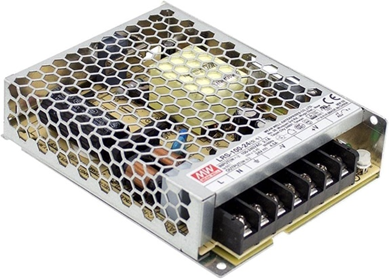
\includegraphics{image/Netzteil.png}
    \caption{Netzteil}
    \label{fig:enter-label}
\end{figure}
